\chapter{Interpreting Medical Images}
\label{ch6}

In modern medical practice, medical image interpretation has largely been conducted by human experts such as radiologists and other physicians. However, owing to the wide variety of medical pathology that may affect human beings, the limitations of human perception, and human fatiguability, an increasing role for computer-aided diagnosis (CAD) in medicine has been recognized. In the past few years, the interest in artificial intelligence has mushroomed within medical image interpretation, driven primarily by remarkable advances in deep learning. As discussed in the previous chapters, advancements in the fields of active learning, model designing, and self-supervised learning have found a myriad of applications in medical image analysis, propelling it forward at a rapid pace. Computers naturally excel at discovering and recognizing intricate patterns from images while also providing quantitative assessments for medical imaging. As a result, CAD systems can overcome human limitations affecting medical image interpretation, allowing physicians to focus more on analytical interpretation tasks. This chapter introduces several distinctive characteristics of medical images, pressing clinical needs for imaging technologies, and existing medical applications.

\section{Characteristics of Medical Images}
\label{ch6:characteristics}

Medical images possess particular characteristics compared with natural images, providing unique opportunities for the application of computer-aided techniques to assist in medical diagnosis. Such particular characteristics provide the basis for imaging research advances that have subsequently been translated into clinically usable products. Below we summarize some of the most distinguished imaging characteristics and discuss how they are exploited to advance computer-aided diagnosis in medical imaging.

\begin{enumerate}
    
    \item \textit{Medical images are created by modalities.} Natural images typically consist of 3-channel (Red, Green, and Blue) images that exist in the visible light spectrum, whereas various modalities are used to create medical images, including computed tomography (CT), magnetic resonance imaging (MRI), positron emission tomography (PET), mammography, ultrasound, radiography, and so on. Each modality uses a portion of the non-visible electromagnetic spectrum (with the exception of ultrasound, which employs sound waves for image creation) to create images for visualizing and identifying certain medical disorders and procedural complications. Certain medical imaging modalities are more conducive for the evaluation of particular disorders than others. For example, abnormalities such as acute active hemorrhage are more readily diagnoseable by intravenous contrast-enhanced CT than MRI, whereas small or subtle lesions such as prostate cancer, uterine cancer, and metastases to the bone and brain may be better shown by MRI. Also, although they may often require the use of ionizing radiation or intravenous contrast administration, cross-sectional techniques, such as CT and MRI, are capable of producing images with substantially richer details than radiography (often colloquially referred to as ``X-rays'').
    
    \item \textit{Medical images possess high dimensionality.} Cross-sectional imaging techniques, such as CT, MRI, and ultrasound, produce three-dimensional images, and when dynamic imaging is performed, a fourth dimension---time---is added. While the world around us is three dimensional, human eyesight is essentially a two-dimensional process. Although various reconstruction algorithms essentially ``simulate'' the 3D world from multiple 2D views, human eyesight nevertheless relies on two-dimensional spatial information processing. When reading a volumetric cross-sectional imaging examination, radiologists must scroll through a stack of images back to mentally ``reconstruct''  the underlying anatomy in three dimensions. This is cumbersome and time-consuming, especially when searching for small lesions, which are only seen on a few images within a large volumetric stack of images, and particularly when an abnormality is similar in appearance to normal anatomies, such as a small lung nodule (which can closely resemble normal pulmonary vessels). To avoid overlooking potentially significant abnormalities, radiologists must scrutinize all aspects of each image contained within a large volumetric stack; nevertheless, it has been well-established through eye-tracking perceptual research that even trained observers fail to visually scan all parts of a medical image~\citep{rubin2015characterizing}. In contrast, computer algorithms can interpret high-dimensional images the same way as 2D images by directly harnessing spatial and temporal information. 
    
    \item \textit{Medical images vary in quality.} Owing to substantial differences among medical imaging equipment manufacturers as well as variable proprietary hardware and software platforms, medical images may vary in quality and content among various institutions as well as within a given institution. Furthermore, acquisition protocol parameters (of which there are numerous considerations that must be addressed for a given application), frequently vary considerably among institutions, even for a given manufacturer and application. Such variability results in ``domain gaps'', both in terms of quality and technical display. These domain gaps are regarded as a major obstacle to the development of robust deep learning methods, often referred to as ``domain shift'' or ``distribution drift''. For example, CT scans performed using 5 mm slice thickness can handicap a model trained using CT scans performed using a 0.75 mm thickness, resulting in deep learning methods with a limited clinical value. While the domain shift problem can be addressed by a universally applied configuration for acquiring medical images across hospitals, such a requisite is unlikely to be adopted. Approaches such as semi-supervised learning, domain adaptation, and federal learning have been explored to address the ``domain shift'' problem.
    
    \item \textit{Medical images convey physical meaning.} The color information in natural images does not usually carry categorical meaning. For instance, a shirt is a shirt no matter what color it is. In contrast, the exact or relative pixel intensity value in a given medical image corresponds to a specific constituent within the human body, particularly for cross-sectional imaging modalities such as CT and MRI. CT images are created by directing ionizing radiation through a body part and counting the relative number of photons absorbed by the tissue traversed by the x-ray beam---a greater number of photons absorbed occurs with denser tissue, such as bone, whereas a greater number of photons transmitted (not absorbed and thus reaching the detector) occurs with less dense tissue, such as lung parenchyma. The commonly used scale to represent the relative amount of X-ray photon absorption at CT is the Hounsfield Units (HU) and reflects tissue density. By convention, an attenuation coefficient of 0 HU is equivalent to the density of water (1 gm/cm$^3$). Air or gas, as may be encountered within the large airways and bowel, has an attenuation coefficient of -1,000 HU, whereas bone, a very dense structure, has an attenuation coefficient of approximately 1000 HU. Other tissues within the human body have attenuation coefficients within this range. For example, fat has a value between -80 and -30 HU, whereas unenhanced muscle has an attenuation coefficient ranging between 35 and 55 HU. This ability to directly measure the density of human tissue enables human experts and computer algorithms to identify both normal human anatomy as well as potential abnormalities. More importantly, the semantics embedded in the pixel intensity is a weak annotation that can be harnessed to facilitate the model to learn the appearance of anatomic structures without extensive manual annotation.
    
    \item \textit{Medical images encode relative location and orientation.} When identifying objects from natural images, their locations are generally not important: a cat is a cat no matter if it appears in the top left or bottom right of the image. In contrast, in medical imaging, the relative location and orientation of a structure and the intrinsic consistency of anatomical relationships are important characteristics that allow recognition of normal anatomy and pathological conditions. The regular and predictable location of various structures in the human body is a valuable characteristic for training deep learning models. Since medical imaging protocols snap patients in fairly consistent and reproducible positions, these methods generate images with great similarity across various equipment manufacturers and facility locations. Therefore, recognizing the stereotypical position and orientation information of human anatomy provides an opportunity to reduce false positive results and improve the accuracy of disease detection and segmentation. Several works have demonstrated the value of this approach by adding location features, modifying objective functions, and constraining coordinates relative to landmarks in images. For instance, employing ultrasound for measurement of carotid arterial intimal-medial thickness for cardiovascular risk stratification, the measurement could be performed at any point along the longitudinal aspect of the vessel, and such variability could adversely affect results and reproducibility. However, it is standard practice to perform this measurement  1 cm beyond a recognizable anatomic landmark---the carotid bulb~\citep{stein2008use}. As a result, the anatomically recognizable carotid bulb provides a contextual constraint for training deep learning methods. 
    
    \item \textit{Medical images encode both scale and distance.} The uncertain distance between camera and object limits precise size measurements in natural images; in contrast, the physical size of a structure is preserved in medical images. Scale is one of the quantitative attributes of standard imaging formats. The size of a pixel in CT, as an example, is often specified in the DICOM header. By obtaining the number of pixels belonging to an object and the pixel scale from the header, the physical scale and distance between normal structures and lesions in the image can easily be computed. This information is a critical feature in the assessment of disease, both by human interpretation and computer-aided diagnosis because the physical size of a lesion influences disease stage, treatment options, and prognosis. Moreover, the lesion size distribution can serve as a statistic to estimate the domain gaps among datasets collected from different equipment manufacturers, facilities, and regions, allowing the creation of more robust models and enhancing the ability to extrapolate computer-aided diagnoses across various medical practices.
    
    \item \textit{Medical images have sparse and noisy labels.} Unlike natural imaging datasets, it is impractical to annotate millions of medical images with a systematic label hierarchy. Most publicly available medical imaging datasets focus on particular anatomic regions and only provide annotation for the object of interest. For example, the KiTS dataset provides annotation only for the kidney, the LiTS dataset for the liver, and the NIH Pancreas-CT dataset for the pancreas. There is no dataset that provides systematic annotation for all visible structures in a medical imaging dataset; existing annotated datasets are either only partially annotated or only annotated on a small scale. Organizing a hierarchical labeling dictionary to address various organs, tissues, and diseases, as well as reflect their spatial relationships in the human body, remains a large limitation for deep learning methods. Moreover, the available annotated images are often associated with noise due to inter-observer and intra-observer variability. That is, different human experts can provide conflicting opinions regarding a given lesion, reflecting inter-observer variability; furthermore, the same expert is likely to produce very different lesion contours over multiple attempts separated in time, reflecting intra-observer variability. Additionally, more severely noisy labels occur if the abnormality has indistinct boundaries, such as diffuse lung diseases. The partial and imperfect annotation compromises model training and results in ambiguous and unreliable results when deep learning methods undergo testing. 

\end{enumerate}


In summary, medical images contain quantitative imaging characteristics---the intensity value and physical size of pixels---that can be used as additional information to enhance deep learning performance. Medical images also present qualitative imaging characteristics---consistent and predictable anatomical structures with great dimensional details---that can provide an opportunity for comprehensive model training. Nevertheless, several characteristics unique to medical images create unmet challenges, such as isolated, discrepant data and partial, noisy labels, that must be addressed through additional investigation.


\section{Clinical Needs}
\label{ch6:clinical_needs}

Computer-aided diagnosis holds a long history, which has been focusing on a key promise: CAD systems are not developed to replace physicians but rather to enhance their capabilities through computer-physician synergy. With deep learning methods elevating numerous CAD systems to human-level precision, the number of clinical needs has been rapidly increasing in recent decades.

\begin{itemize}
    \item \textit{Medical image classification} refers to classifying what type of lesion is contained in an image. Such classification may be binary (\eg benign or malignant) or multi-class (various types of lesions). The annotation for classification tasks is to assign one or a few labels to an image or a study.
    
    \item \textit{Disease localization and detection} refer to identifying the location of specific lesions. Their difference is subtle: localization aims to locate a single lesion, while detection aims to find all lesions in the image. The annotation for detection and localization provides both the specific location and the scale of the disease with a bounding box.
    
    \item \textit{Medical image segmentation} refers to creating a pixel-wise mask of the organ/lesion in the image. Segmentation can ease the analysis by measuring more accurate and desirable imaging biomarkers. The annotation for segmentation tasks is to assign every pixel in an image to at least one class.
    
    \item \textit{Medical image registration} refers to aligning the spatial coordinates of one or more images into a standard coordinate system. Image registration plays an important role in disease prognosis by establishing correspondence among multiple scans taken from different time points. 
    
    \item \textit{Medical image reconstruction} refers to producing images suitable for human interpretation from raw data obtained by imaging devices, such as CT or MRI scanners. A fast and high-quality radiological image reconstruction will substantially reduce radiation exposure and doses of intravenous contrast material.
    
    \item \textit{Medical image enhancement} refers to adjusting the intensity of an image for better visualization or further analysis. Such enhancement includes denoising, super-resolution, artifact removal, MR bias field correction, and image harmonization.
    
    \item Other tasks include: \textit{landmark detection}, \textit{image or view recognition}, \textit{automatic report generation}, etc.

\end{itemize}


In this dissertation, we mainly focus on the tasks of image classification and segmentation, with some other clinical needs such as disease detection and CIMT thickness measurement. Our goal is to minimize the annotation cost associated with these tasks while maintaining comparable or even higher performance. We have further elaborated on the specific imaging datasets in Appendix~\ref{ap1}.





\section{Medical Application: A Case Study of PE CAD}
\label{ch6:medical_applications}

Interest in implementing deep learning methods in computer-aided diagnosis systems has increased tremendously in the past decade due to the promising, or even super-human, performance for various medical applications. This section provides a case study for conducting a medical application that involves deep learning, from curating the structure of data and annotation, to developing the system and validating the performance. Specifically, the objective is to demonstrate the annotation-efficiency of our devised techniques in several key facets of the CAD system in practice. We illustrate the step-by-step workflow using the application of detecting pulmonary embolism from CTPA scans. The idea of implementing deep learning methods into computer-aided diagnosis systems can be adapted to many other medical applications that require automated medical image analysis.

%##############################################################################################
\begin{figure}[t]
\begin{center}
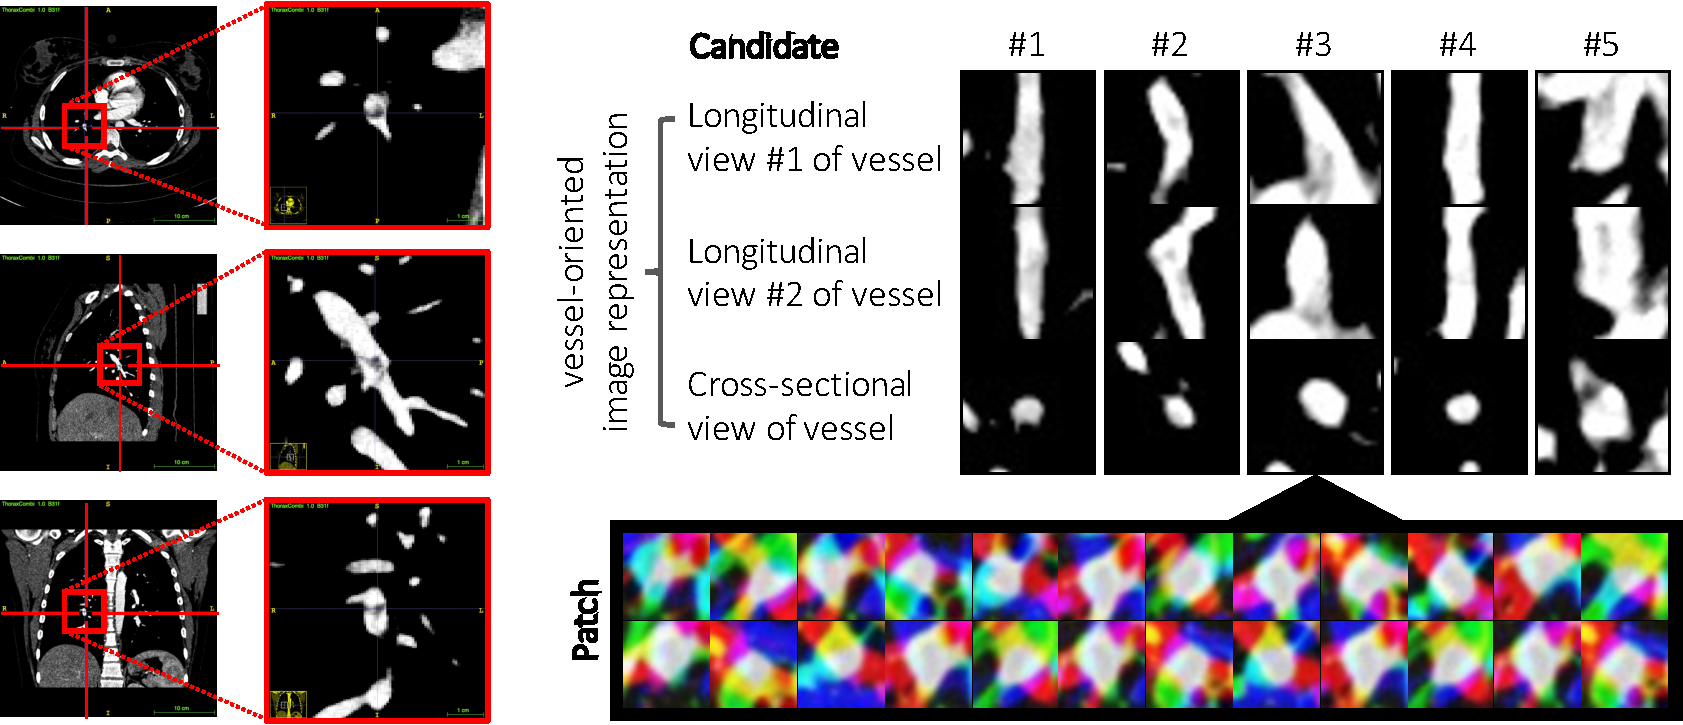
\includegraphics[width=1.0\linewidth]{Figures/CH6/fig_pe_visualization.pdf}
\end{center}
\caption[Examples of Pulmonary Embolism in CTPA Images]{(a) The typical appearance of pulmonary embolism in the CTPA scan, presented from an axial, coronal, and sagittal views. (b) Five different pulmonary embolism candidates in the vessel-oriented image representation~\citep{tajbakhsh2015computer}. It was adopted in this work because it achieves great classification accuracy and accelerates CNN training convergence.}
\label{ch6:fig:pe_visualization}
\end{figure}
%##############################################################################################

\subsection{Pulmonary Embolism}
\label{ch6:medical_applications:pe_introduction}

Pulmonary Embolism (PE) is a major national health problem, which is responsible for 100,000$\sim$200,000 deaths annually in the United States~\citep{pauley2019age}, representing the third most common cause of cardiovascular death after myocardial infarction and stroke~\citep{martin2020time}. A PE is a condition in which a thrombus (often colloquially referred to as a ``blood clot'') travels to the lungs, often from a lower extremity venous source, producing a blockage of the pulmonary arteries within the lungs. The mortality rate of untreated PE may approach 30\%~\citep{calder2005mortality}, but it decreases to as low as 2\% with early diagnosis and appropriate treatment~\citep{sadigh2011challenges}. CT pulmonary angiography (CTPA) is the primary means for PE diagnosis, wherein a radiologist carefully traces each branch of the pulmonary artery for any suspected PEs. PEs appear as ``filling defects'' within enhanced pulmonary arteries following the administration of intravenous contrast, as shown in~\figureautorefname~\ref{ch6:fig:pe_visualization}(a). However, CTPA interpretation is a time-consuming task, of which accuracy depends on human factors, such as attention span and sensitivity to the visual characteristics of PEs. Computer-aided PE detection can have a major role in improving the diagnostic capability of radiologists and decreasing the reading time of CTPA scans.

We developed our computer-aided PE detection system by using an in-house dataset from ASU-Mayo~\citep{tajbakhsh2019computer}, which consists of 121 CTPA scans with a total of 326 emboli\footnote{I thank Jae Y. Shin for organizing and pre-processing the PE dataset.}. The dataset provides the spatial coordinates of each emboli in the scan. The dataset is divided at the patient-level into a training set (71 patients) and a test set (50 patients). To study the robustness and generalizability of the algorithm, we have also evaluated our system using 20 CTPA scans from the CAD-PE competition\footnote{\href{http://www.cad-pe.org/}{http://www.cad-pe.org/}}. Our computer-aided PE detection system consists of two stages to detect PEs from images: (1) candidate generation and (2) false positive reduction. These two stages have also been widely used in most existing disease detection systems. In the following sections, we describe the methodology and performance for each stage in detail.





\subsection{Generating Pulmonary Embolism Candidates}
\label{ch6:medical_applications:candidate_generation}

We use an unsupervised approach for candidate generation, consisting of heuristic lung segmentation and the tobogganing algorithm~\citep{fairfield1990toboggan}. In a chest CTPA scan, lungs appear darker than their surrounding. To segment lungs from the scan, we first clip voxel intensity values using a threshold of -400, resulting in a binary volume wherein the lungs and other dark regions appear white. Then, we perform a closing operation to fill all dark holes in the white area. To exclude non-lung areas, we perform a 3D connected component analysis and remove the components with small volumes or a large length ratio between the major and minor axes. The purpose of segmenting the lungs is to reduce the computational time and the number of false positives for the toboggan algorithm. Since peripheral PEs only appear in pulmonary arteries, there is no need to search for PE candidates outside the lungs. The tobogganing algorithm is then applied only to the lung area, generating the PE candidate coordinates that we will then use to crop sub-volumes from the CTPA scan. This procedure of candidate generation was firstly designed by~\citet{tajbakhsh2015computer}. 


We directly applied their PE candidate generator to the dataset, resulting in a total of 8,585 PE candidates, wherein 863 were true positives and 7,722 were false positives. There are 326 unique emboli annotated in our dataset. Since multiple detections can be generated from a large PE, the number of true positives is greater than the number of unique emboli. \citet{tajbakhsh2015computer} reported a sensitivity of 93\% with, on average, 65.8 false positives per patient for the entire candidate generation stage.


\begin{table}[t]
\centering
\footnotesize
\caption[Models Genesis with 3D VOIR Perform the Best in PE Detection]{
We evaluate vessel-oriented image representation (VOIR)~\citep{tajbakhsh2019computer} in comparison with 2D, 2.5D, and 3D solutions for the task of reducing PE false positives. Our comprehensive experiments have demonstrated that: (1) the vessel-oriented image representation exceeds the regular image representation; (2) 3D volume-based inputs offer higher performance than 2.5D orthogonal inputs, which in turn work better than 2D slice-based inputs; (3) Models Genesis consistently outperform models learning from scratch. Overall, the best performance is obtained by Models Genesis trained with 3D volume-based VOIR inputs. The entries in bold highlight the best results achieved by different model input formations. All of the results in the table are candidate-level AUC (Area Under the ROC Curve), including the mean and standard deviation (mean$\pm$s.d.) across ten trials.
}
\label{ch6:tab:voir_nonvoir}
\begin{tabular}{p{0.29\linewidth}P{0.2\linewidth}P{0.2\linewidth}P{0.2\linewidth}}
    \hline
    Task: \texttt{ECC} (w/o VOIR) & Random & Models ImageNet & Models Genesis \\
    \hline
    2D slice-based input & 60.33$\pm$8.61 & 62.57$\pm$8.04 & \textbf{62.84$\pm$8.78} \\
    2.5D orthogonal input & 71.27$\pm$4.64 & \textbf{78.61$\pm$3.73} & 78.58$\pm$3.67 \\
    3D volume-based input & 80.36$\pm$3.58 & n/a & \textbf{88.04$\pm$1.40} \\
    \hline
    Task: \texttt{ECC} (w/t VOIR) & Random & ImageNet & Genesis \\
    \hline
    2D slice-based input & 86.16$\pm$1.94 & 86.83$\pm$0.97 & \textbf{87.43$\pm$1.34} \\
    2.5D orthogonal input & 87.29$\pm$3.25 & 88.04$\pm$0.78 & \textbf{88.32$\pm$1.70} \\
    3D volume-based input & 92.01$\pm$0.98 & n/a & \textbf{92.81$\pm$0.47} \\
    \hline
    \end{tabular}
\end{table}


\subsection{Reducing Pulmonary Embolism False Positives}
\label{ch6:medical_applications:false_positive_reduction}

The previous stage generates coordinates that indicate where the PE candidate is located. We crop sub-volumes based on the location, so that the PE candidate will appear in the center of each sub-volume. The sub-volume has a physical size of 20$\times$20$\times$20 mm and then resized into 64$\times$64$\times$64 pixel. To conduct a fair comparison with the prior studies~\citep{zhou2017fine,tajbakhsh2016convolutional,tajbakhsh2019computer}, we compute candidate-level AUC (Area Under the ROC Curve) for classifying true positives and false positives. 


Compared with \citet{tajbakhsh2019computer}, we have advanced the methodology and yielded significant performance gains in three aspects (see~\tableautorefname~\ref{ch6:tab:voir_nonvoir}).

\begin{enumerate}

    \item \textit{Extending VOIR into the 3D version.} 
    In general, emboli can affect pulmonary arteries in any orientation, exhibiting a significant variation in PE appearance (see~\figureautorefname~\ref{ch6:fig:pe_visualization}(a)). This complicates the classification task and hinders the effective utilization of deep learning methods. To implement vessel alignment, we first apply principal component analysis (PCA) to voxel intensities for estimating the vessel's orientation. Then, we rotate scan planes in alignment with the vessel longitudinal axis, resulting in images with standardized appearance, wherein emboli consistently appear as elongated structures in the longitudinal vessel view and as circular structures in the cross-sectional view (see~\figureautorefname~\ref{ch6:fig:pe_visualization}(b)). This interpolation scheme guided by the vessel axis has the effect of maximally revealing the filling defects, thereby facilitating PE diagnosis for both radiologists and computers. We have implemented VOIR in both 2D (following~\citet{tajbakhsh2019computer}) and 3D\footnote{I thank Douglas Amoo-Sargon for implementing 3D VOIR in the PE dataset.}, demonstrating that the vessel-oriented image representation exceeds the regular image representation.
    
    \item \textit{Utilizing three-dimensional models and data.}
    While adopting 3D models to process 3D volumetric data may appear to be a natural choice, it occurs at a substantial computational cost, lack of sufficient data, and risk of overfitting. As a result, several alternative strategies were proposed to reformat 3D applications into 2D problems. For instance, \citet{ben2016fully,sun2017multiphase} formulated regular 2D inputs by extracting adjacent axial slices (refer to as 2D slice-based input). A more advanced strategy, presented in~\citet{prasoon2013deep,roth2014new,roth2015improving}, is to extract axial, coronal, and sagittal slices from volumetric data (refer to as 2.5D orthogonal input). These reformatted 2D solutions can generate a large number of data and benefit from 2D pre-trained ImageNet. However, 2D solutions inevitably sacrifice the rich spatial information in 3D volumetric data and large capacity of 3D models. As the computer power increased and pre-trained 3D models developed in recent years, the interest is shifting back to 3D techniques, with several emerging evidences~\citep{zhou2021models,isensee2021nnu} indicating that 3D applications are better to be addressed in 3D. Our experimental results also suggest that, with the same initialization and vessel orientation, 3D volume-based inputs offer higher performance than 2.5D orthogonal inputs, which in turn work better than 2D slice-based inputs.
    
    \item \textit{Initializing models with Models Genesis.}
    Training a deep model from scratch is difficult because it requires a large amount of labeled training data and a great deal of expertise to ensure proper convergence. Fine-tuning Models ImageNet has become the most practical adoption for deep learning applications in medical imaging to ease the training procedure~\citep{shin2016deep,tajbakhsh2016convolutional}. On the other hand, Models ImageNet may give suboptimal initialization in the medical imaging domain~\citep{raghu2019transfusion}, as they were pre-trained from only natural images; it is associated with a large domain gap for medical images. We pre-train Models Genesis in the same domain to reduce this domain gap. Our Models Genesis 2D offer similar performance to Models ImageNet. This result is encouraging because our Models Genesis 2D were developed without using any manual annotation, while Models ImageNet demand more than fourteen million annotated images. More importantly, Models ImageNet only provide 2D models, which cannot handle 3D data directly, while Models Genesis can be pre-trained in both a 2D and 3D manner. Our results show that Models Genesis secure great performance gain (10\% improvement without VOIR and 4\% with VOIR) in comparison with Models ImageNet. Overall, we conclude that Models Genesis consistently outperform models learning from scratch and achieve the best performance when using 3D VOIR sub-volumes as input.
    
    
\end{enumerate}



%%%%%%%%%%%%%%%%%%%%%%%%%%%%%%%%%%%%%%%%%%%%
% \begin{landscape}
% \thispagestyle{empty}

\begin{sidewaysfigure}
\begin{center}
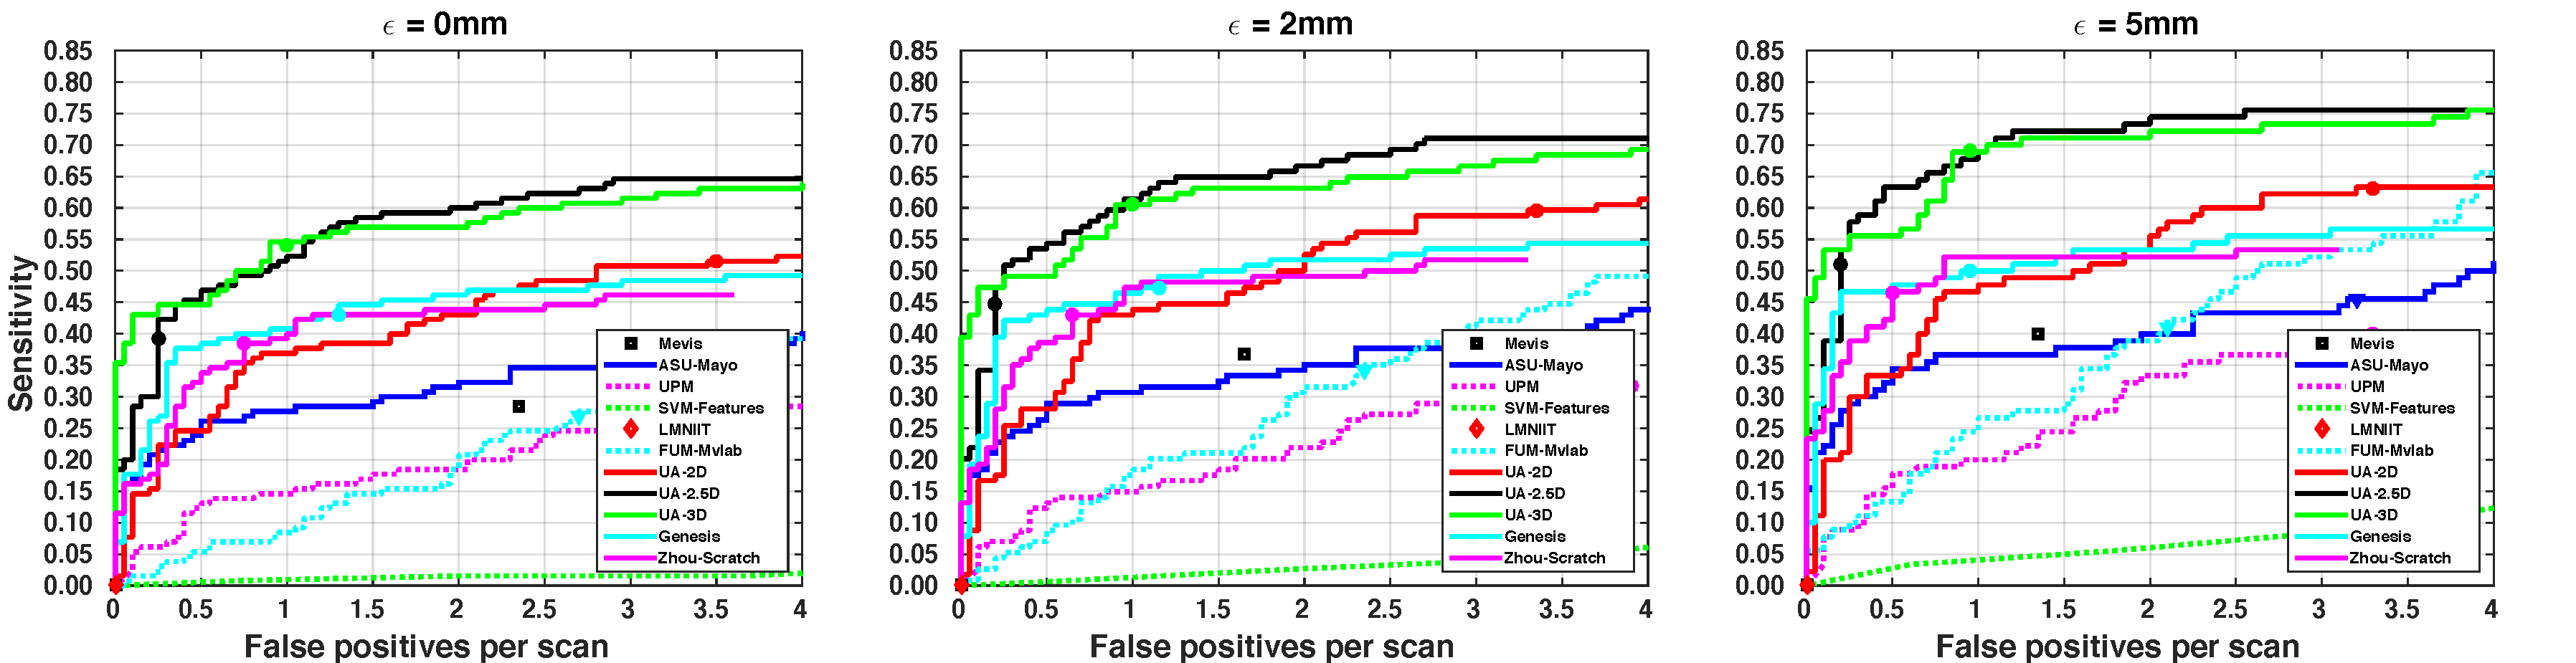
\includegraphics[width=1.0\columnwidth]{Figures/CH6/fig_pe_cad.pdf}
\end{center}
\caption[Comparison of Our PE CAD System with the State of the Arts]{
We have compared the top participating teams of the CAD-PE competition~\citep{gonzalez2020computer}. For each method, the Free‐Response Operating Characteristic (FROC) curves are plotted. 
Our PE CAD was directly evaluated on the 20 CTPA test scans, without using any training scans provided by the competition. 
$\epsilon$ denotes the localization error. That is, a detection is considered a true positive as long as the detection falls within $\epsilon$ distance from the ground truth for PE. The performance at $\epsilon$ = 0 mm provides greater benefits for clinical applications than at 2mm and 5 mm. As reported, our PE CAD (\texttt{Genesis}) is ranked third among the participating teams, achieving a sensitivity of 46\% at 2 false positives per scan ($\epsilon$ = 0 mm). 
This sensitivity is substantially higher than our previous method, which holds a sensitivity of 33\%  (\texttt{ASU-Mayo})~\citep{tajbakhsh2019computer}, highlighting the importance of 3D VOIR and Models Genesis for PE detection. 
We should note that the leading solutions (\texttt{UA-2.5D} and \texttt{UA-3D}) have not only been trained on the 20 training scans, but also had access to an extended training dataset with 51 additional CTPA scans. 
Therefore, our PE CAD is reasonably competitive compared to the state of the art. 
}
\label{ch6:fig:pe_cad}
\end{sidewaysfigure}

% \fillandplacepagenumber
% \end{landscape}
%%%%%%%%%%%%%%%%%%%%%%%%%%%%%%%%%%%%%%%%%%%%


\subsection{Comparing with the State of the Art}

To further examine the robustness of our computer-aided PE detection system, we have participated in the CAD-PE competition\footnote{I thank Nima Tajbakhsh and Jae Y. Shin for generating PE candidates from the competition dataset; German Gonzalez Serrano for organizing the CAD-PE competition and evaluating our system with other participating teams.}. All participating teams can use 20 training scans provided by the competition to develop their systems, and the final performance is evaluated on the additional 20 unseen scans. As shown in~\figureautorefname~\ref{ch6:fig:pe_cad}, our system (\texttt{Genesis}) is ranked third among the participating teams. The top two winners of the competition, \texttt{UA-3D} and \texttt{UA-2.5D}, have utilized an extended training set released by the competition organizers; therefore, their systems are significantly better than others. On the other hand, we directly took the unseen test scans to evaluate our system, which was developed even without using the 20 training scans from the competition. As seen, our system's performance is fairly robust to the different datasets. Considering the potential domain gap between the CAD-PE competition and our in-house dataset, we also anticipate a better performance once adapting our system to the CAD-PE training set in the future. The \texttt{ASU-Mayo} was our previous submission, which used the 2D VOIR approach~\citep{tajbakhsh2019computer}, a consistent, compact, and discriminative image representation to improve the perception of PE. Our current system, compared with \citet{tajbakhsh2019computer}, has made three advancements: (1) extending VOIR to the 3D version, (2) utilizing three-dimensional models and data, and (3) initializing models with Models Genesis. Consequently, the enhanced system achieves a significantly higher sensitivity of 46\% at 2 false positives per scan ($\epsilon$ = 0 mm), increasing the sensitivity by over 10\% than the previous system.


\section{Discussion \& Conclusion}
\label{ch6:discussion}

\subsection{What Is the Current State of Clinical PE CAD?}
\label{ch6:discussion:current_state_of_pe_cad}

The computer-aided pulmonary embolism detection is an illustrative example of how deep learning methods have been integrated into clinical image interpretation. With an estimated 180,000 deaths per year in the United States, the rapidly increasing CTPA examinations far exceed the availability of subspecialty trained cardiopulmonary radiologists~\citep{horlander2003pulmonary}. To address the unmet need for interpretation, general radiologists are also assigned to look through some of the examinations.
Accurately interpreting CTPA examinations requires significant training and experience, so the discordance between cardiopulmonary and general radiologists may exceed 25\% if they interpret the same examination~\citep{hutchinson2015overdiagnosis}. Due to inaccurate interpretations, including false-negative studies (failure to detect emboli) and false-positive studies (diagnosing emboli that are not present, or ``overdiagnosis’’), there is a significant risk of morbidity and mortality for patients. 

Deep learning methods have been developed to assist radiologists with the task of PE detection and exclusion. Several studies suggest that radiologists who use current CAD systems can improve the sensitivity from 77$\sim$94\% to 92$\sim$98\%~\citep{das2008computer,wittenberg2011impact,blackmon2011computer,wittenberg2013computed}. 
One particular system, developed by AIDOC medical (Tel Aviv, Israel), has recently been adopted by Mayo Clinic\footnote{I thank Michael B. Gotway for sharing the clinical experience of PE CAD in Mayo Clinic.}. Once a CTPA examination is transferred from the CT scanner to radiologists for interpretation, the system will perform the task of PE detection and exclusion in the backend. This system runs ``silently'' in the background and determines results as either negative or positive for PE. If positive, a pop-up window will localize the embolus for radiologist confirmation. In a study by~\citet{weikert2020automated}, the AIDOC algorithm showed a sensitivity of 92.7\% on a per-patient basis with a false positive rate of 3.8\%, or 0.12 false-positive detection. Most notably, the average processing time for the algorithm was 152 seconds, but typically this processing occurs while the data is being transferred from the CT scanner to the picture archiving communication system. Thus, the images are not completely available for radiologists to review immediately. An additional 25 seconds is required for case uploading~\citep{weikert2020automated}. In practice, the AIDOC system analysis is either complete and ready for review when the study is opened by the radiologist, or the case is being actively processed. The examination is open for interpretation and the results are commonly available before the radiologist completes the review of the study. 
Such a PE CAD system cannot, and was not designed to, substitute the doctor, but it definitely makes radiologists better and faster decision makers, playing a supporting and final interpretative role in medical diagnosis.


\subsection{Conclusion and Broader Impacts}
\label{ch6:discussion_conclusion:conclusion_broader_impacts}

The introduction of deep learning methods in clinical medicine, particularly diagnostic imaging, has rapidly stimulated many medical applications in recent years. In this chapter, several important characteristics of medical images and pressing clinical needs are reviewed to highlight their strengths and limitations. Accordingly, the techniques we devised were mainly inspired by these imaging characteristics, while the medical applications we chose were deeply motivated by the clinical needs. Furthermore, we have presented our end-to-end CAD system for pulmonary embolism detection as an example of how deep learning methods address clinical problems. We have illustrated the annotation efficiency in several key facets of the system and demonstrated our system's robustness in the CAD-PE competition. Numerous other deep learning applications are already available to assist radiologists with interpreting a wide variety of disorders from images, functioning as a ``second reader''. These applications hold promise both for providing increased accuracy through enhanced detection and specificity, and for mitigating the workloads experienced by radiologists due to the rise of advanced imaging techniques. 


% \section*{Acknowledgements}

% I thank Michael B. Gotway for revising this chapter and sharing the clinical experience of PE CAD in Mayo Clinic; Jae Y. Shin for organizing and pre-processing the PE dataset; Douglas Amoo-Sargon for implementing 3D VOIR to the PE dataset; Nima Tajbakhsh for generating PE candidates from the competition dataset; German Gonzalez Serrano for organizing the CAD-PE competition and evaluating our system with other participating teams; Jianming Liang for providing constructive advises.


% \subsection{Acquiring annotations in candidate-level or patient-level?}

% \subsection{Computer-aided diagnosis or automated computer diagnosis?}

% \subsection{What would be the clinically acceptable performance?}

% \subsection{On which aspects can computers impact the most?}
